  Для взаимодействия с монитором светимости и детальной визуализации данных был разработан графический интерфейс. Для реализации графического интерфейса используется язык программирования C++ и кроссплатформенный фреймворк Qt. Также использовался шаблон проектирования MVC, который легко реализуется благодаря механизму сигналов и слотов, которые являются способом взаимодействию между объектами используемому в Qt. Сигналы это события посылаемые от объекта к объекту, а слоты это методы, которые обрабатывают данное событие.\par
\begin{figure}[htp]
  \centering
  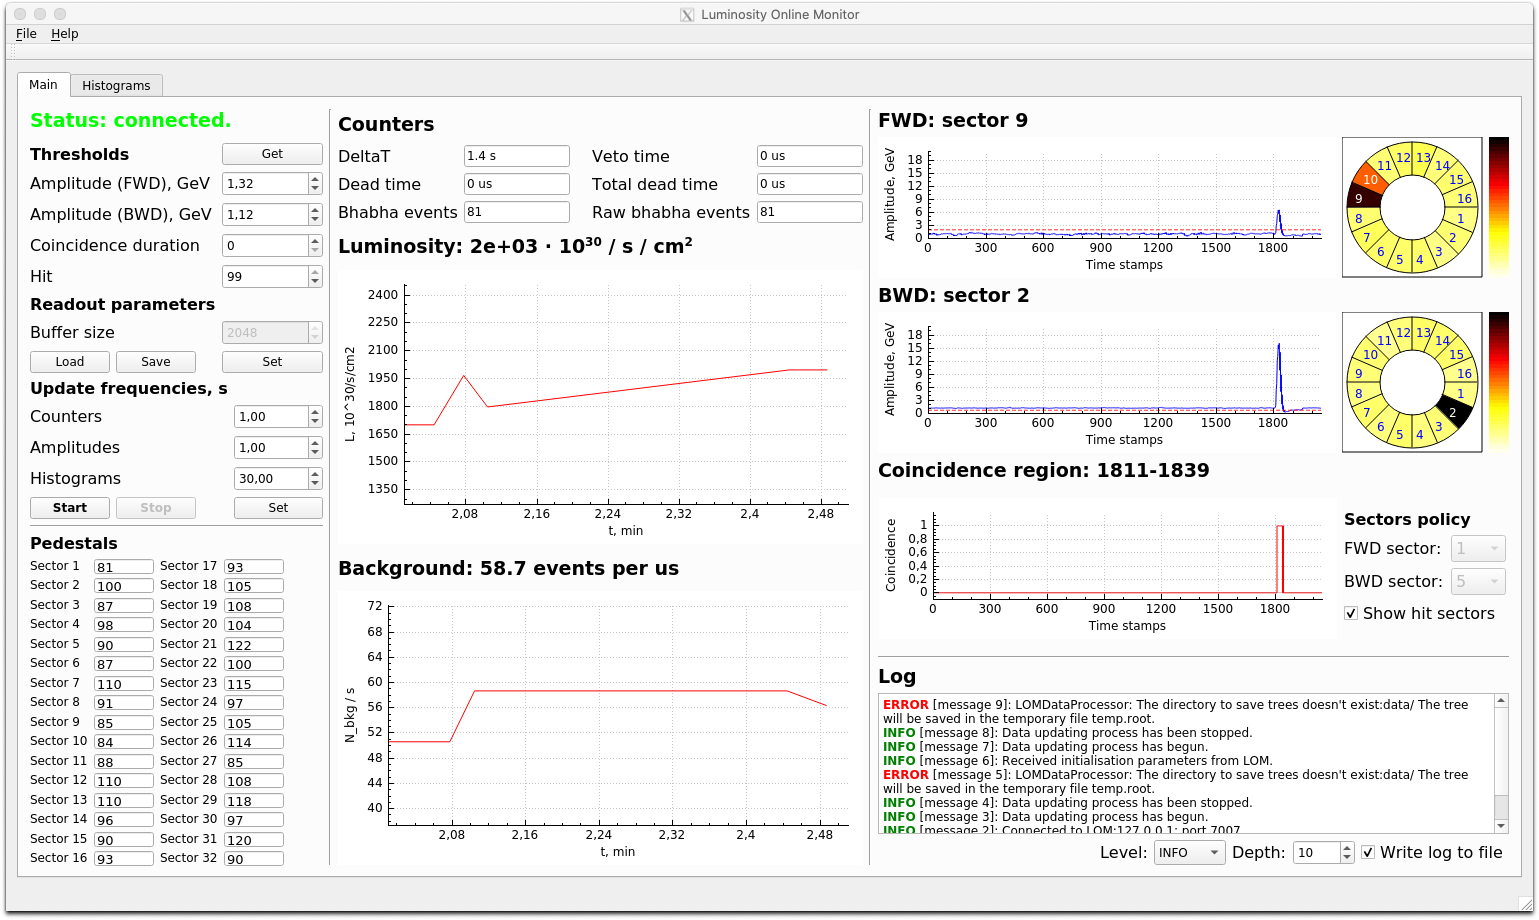
\includegraphics[width=\textwidth]{GUI3}
  \caption{Графический интерфейс для отображения данных с монитора светимости}
  \label{fig:galaxy}
\end{figure}
  На рисункеХ представлен графический интерфейс монитора светимости. Весь интерфейс разделен на 6 частей:
\begin{itemize}
  \item Конфигурация монитора светимости
    \begin{itemize}
      \item Отображаются амплитудные пороги при превышении которых событие считается полезным
      \item Имеется возможность считать регистры с монитора светимости в котрых заданы значения данных порогов
      \item Задать региан совпадения, если совпадение больше заданной величины, то можно считать событие полезным
      \item Установить частоту обновлений счетчиков, форм сигналов и гистограмм
    \end{itemize} 
  \item Отображение пьедесталов. Отображает значения пьедесталов и считывает значения с частотой 1Гц
  \item Счетчики. Отображаются следующие значения
    \begin{itemize}
      \item DeltaT
      \item Мертвое время 
      \item Общее мертвое время
      \item Количство событий $e^+e^-$ рассеяния
      \item Количество фоновых событий
      \item Время инжекции
    \end{itemize}
  \item Отображение светимости. Отображаются:
    \begin{itemize}
      \item Мгновенная светимость
      \item Фоновые события
    \end{itemize}
  \item Визуализация амплитуд
  \begin{itemize}
    \item Представлены изображения секторов и тепловой картой отображаются сектора в которых амплитуды превысили пороговое значение
    \item Отображаются формы сигналов в секторах
    \item Имеется возможность отображать конкретный сектор переднего и заднего торца
    \item Имеется возможность отображать сектора в которых зарегистрировано превышение порогового значения амплитуды
    \item Отображается регион совпадения.
  \end{itemize}
  \item Логирование событий. Отображается журналирование событий
    \begin{itemize}
      \item INFO журналирование информационных событий, таких как подключение к монитору светимости
      \item ERROR журналирование только ошибок
      \item DEBUG детальное журналирование всех событий, например получение конкретных данных с монитора светимости
    \end{itemize}
\end{itemize}\par
  Также в графическом интерфейсе записываются светимости и формы сигналов в течение одного часа и по истечению данного времени сохраняются в файл, для последующей визуализации любого момента времени. Планируется интегрировать данную возможность с веб сервером.
